% !TEX TS-program = pdflatex
% !TEX encoding = UTF-8 Unicode

% This is a simple template for a LaTeX document using the "article" class.
% See "book", "report", "letter" for other types of document.

\documentclass[11pt]{article} % use larger type; default would be 10pt

\usepackage[utf8]{inputenc} % set input encoding (not needed with XeLaTeX)

%%% Examples of Article customizations
% These packages are optional, depending whether you want the features they provide.
% See the LaTeX Companion or other references for full information.

%%% PAGE DIMENSIONS
\usepackage{geometry} % to change the page dimensions
\geometry{a4paper} % or letterpaper (US) or a5paper or....
% \geometry{margin=2in} % for example, change the margins to 2 inches all round
% \geometry{landscape} % set up the page for landscape
%   read geometry.pdf for detailed page layout information

\usepackage{graphicx} % support the \includegraphics command and options

% \usepackage[parfill]{parskip} % Activate to begin paragraphs with an empty line rather than an indent

%%% PACKAGES
\usepackage{booktabs} % for much better looking tables
\usepackage{array} % for better arrays (eg matrices) in maths
\usepackage{paralist} % very flexible & customisable lists (eg. enumerate/itemize, etc.)
\usepackage{verbatim} % adds environment for commenting out blocks of text & for better verbatim
%\usepackage{subfig} % make it possible to include more than one captioned figure/table in a single float
% These packages are all incorporated in the memoir class to one degree or another...

%CUSTOM PACKAGES
\usepackage{listings}
\usepackage{color}
\usepackage{caption}
%\usepackage{subcaption}
\usepackage{tabu}
\usepackage{subcaption}

%Customize lists
\usepackage{enumitem}
%\renewcommand{\labelitemi}{$\blacksquare$}
\renewcommand\labelitemii{$\circ$}
 
\definecolor{codegreen}{rgb}{0,0.6,0}
\definecolor{codegray}{rgb}{0.5,0.5,0.5}
\definecolor{codepurple}{rgb}{0.58,0,0.82}
\definecolor{backcolour}{rgb}{0.95,0.95,0.92}
 
\lstdefinestyle{mystyle}{
    backgroundcolor=\color{backcolour},   
    commentstyle=\color{red},
    keywordstyle=\color{\color{cyan}},
    numberstyle=\tiny\color{codegray},
    stringstyle=\color{codepurple},
    basicstyle=\footnotesize\ttfamily,
    breakatwhitespace=false,         
    breaklines=true,                 
    captionpos=b,                    
    keepspaces=false,                 
    numbers=left,                    
    numbersep=5pt,                  
    showspaces=false,                
    showstringspaces=false,
    showtabs=false,                  
    tabsize=2
}

\lstset{style=mystyle}

%%% HEADERS & FOOTERS
\usepackage{fancyhdr} % This should be set AFTER setting up the page geometry
\pagestyle{fancy} % options: empty , plain , fancy
\renewcommand{\headrulewidth}{0pt} % customise the layout...
\lhead{}\chead{}\rhead{}
\lfoot{}\cfoot{\thepage}\rfoot{}

%%% SECTION TITLE APPEARANCE
\usepackage{sectsty}
\allsectionsfont{\sffamily\mdseries\upshape} % (See the fntguide.pdf for font help)
% (This matches ConTeXt defaults)

%%% ToC (table of contents) APPEARANCE
\usepackage[nottoc,notlof,notlot]{tocbibind} % Put the bibliography in the ToC
\usepackage[titles,subfigure]{tocloft} % Alter the style of the Table of Contents
\renewcommand{\cftsecfont}{\rmfamily\mdseries\upshape}
\renewcommand{\cftsecpagefont}{\rmfamily\mdseries\upshape} % No bold!

%%% END Article customizations

%%% The "real" document content comes below...

%%%%%%%%%%%%%%%%%%%%%%%%%%%%%%%%%%%%%%%%%%%%%%%%%%%%%%%%%%%%%%%%%%%%%%

\title{BoloCalc User Manual \\ Version 1.0}
\author{Charles Hill, UC Berkeley}
\date{Last Updated: 2018-06-05}

\begin{document}
\maketitle

\tableofcontents
\pagebreak

%%%%%%%%%%%%%%%%%%%%%%%%%%%%%%%%%%%%%%%%%%%%%%%%%%%%%%%%%%%%%%%%%%%%%%

\section{Quick Start}
\label{sec:quick}

This section quickly covers whats needed to get \texttt{BoloCalc} up and running.

%%%%%%%%%%%%%%%%%%%%%%%%%%%%%%%%%

\subsection{System Requirements}
\label{sec:sysreq}

\texttt{BoloCalc} is to be run on a Linux and needs the following installed

\begin{enumerate}
\item Python v2.7.2
\item Numpy v1.8 or above
\end{enumerate}

%%%%%%%%%%%%%%%%%%%%%%%%%%%%%%%%%

\subsection{Code location}
\label{sec:source}

\texttt{BoloCalc} is stored on Charles Hill's GitHub account \texttt{chill90} within the repository \\ \texttt{chill90/BoloCalc}. To clone a local copy of the repository, make sure that you have Git installed on your machine and run

\begin{lstlisting}
	git clone https://github.com/chill90/msCorr.git
\end{lstlisting}

All executables are stored at in the top-most directory

\begin{lstlisting}
	~/BoloCalc/
\end{lstlisting}

and all libraries are stored in the \texttt{src/} directory

\begin{lstlisting}
	~/BoloCalc/src/
\end{lstlisting}

%%%%%%%%%%%%%%%%%%%%%%%%%%%%%%%%%

\subsection{Running \texttt{mappingSpeed.py}}
\label{sec:runms}

The primary \texttt{BoloCalc} executable is called \texttt{mappingSpeed.py}, which calculates optical power, noise-equivalent power (NEP) contributions from photon noise, bolometer thermal carrier noise, readout noise, per-detector noise-equivalent temperature (NET), array NET, mapping speed, and map depth, given some instrument configuration. \texttt{mappingSpeed.py} takes as input an experiment configuration directory, which is stored in \texttt{BoloCalc/Experiments} and has the following structure:

\begin{lstlisting}
	CHillCalc/
	 |-- Experiements/
	 |    |-- Experiment 1/
	 |    |    |-- Experiment Design 1/
	 |    |    |-- Experiment Design 2/
	 |    |    |-- ...
	 |    |-- Expierment 2/
	 |    |-- ...
\end{lstlisting}
			
To calculate the sensitivity an experiment, pass its \texttt{Experiment Design} directory to \texttt{mappingSpeed.py}. The \texttt{BoloCalc} repository comes with an example  experiment that can be used to get started: 

\begin{lstlisting}
	BoloCalc$ python2.7 mappingSpeed.py Experiments/ExampleExp/V0/	
\end{lstlisting}

By default upon download, this execution will calculate one experiment realization, which should be shown by the status bar. The simulation parameters can be tuned in the \texttt{BoloCalc/config/simulationInputs.txt}

\begin{figure}[h!]
	\centering
	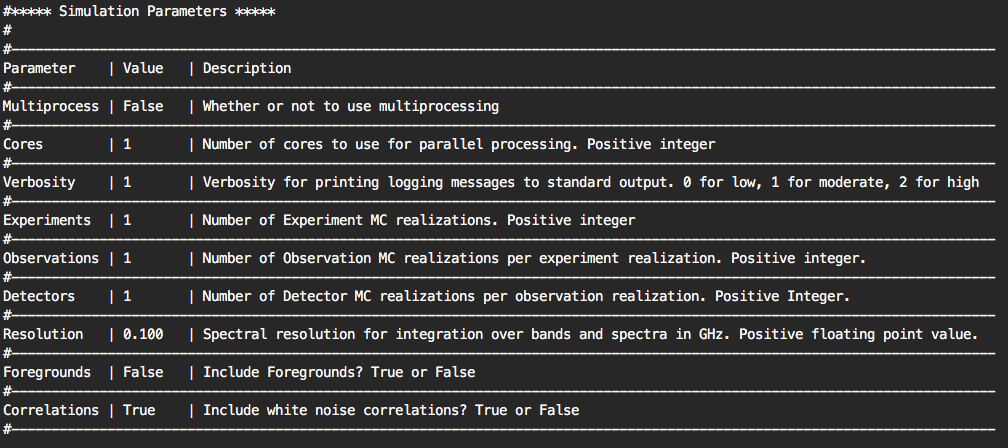
\includegraphics[width=1.0\textwidth]{SimulationInputs_Example}
\end{figure}

After it has finished running, \texttt{mappingSpeed.py} generates several tables that display the calculated quantites for the simulated instrument. All files are named \texttt{sensitivity.txt}, but each is located at a different level of the experiment and therefore contains different information.

\begin{itemize}[noitemsep,topsep=0pt]
	\item \texttt{Experiments/ExampleExp/V0/sensitivity.txt}: contains the sensitivity combined by observation frequency of all telescopes in this experiment.
	\item \texttt{Experiments/ExampleExp/V0/Tel/sensitivity.txt}: contains the sensitivity combined by observation frequency of all cameras in this telescope.
	\item \texttt{Experiement/ExampleExp/V0/Tel/Cam/sensitivity.txt}: containst the sensitivity for each observation frequency in this camera.
\end{itemize}

%%%%%%%%%%%%%%%%%%%%%%%%%%%%%%%%%

\subsection{Running \texttt{mappingSpeed\_vary.py}}
\label{sec:runmsv}

The other \texttt{BoloCalc} executable is called \texttt{mappingSpeed\_vary.py}, which calculates the same output parameters as \texttt{mappingSpeed.py} (Section \ref{sec:runms}) given a passed instrument configuration

\begin{lstlisting}
	BoloCalc$ python2.7 mappingSpeed_vary.py Experiments/ExampleExp/V0/	
\end{lstlisting}

 and parameters to be varied, which are stored in \texttt{BoloCalc/config/paramsToVary.txt}. An example of the 

\begin{figure}[h!]
	\centering
	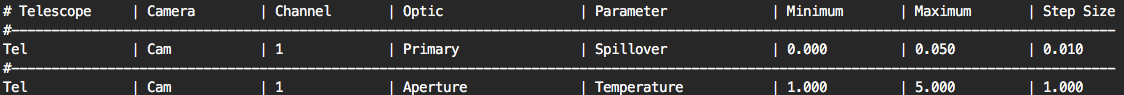
\includegraphics[width=1.0\textwidth]{ParamsToVary_Example}
\end{figure}

Parameters are defined by row and have the following descriptors, which are organized by column:

\begin{itemize}[noitemsep,topsep=0pt]
	\item Column 1: Telescope in which the parameter is defined
		\begin{itemize}[noitemsep,topsep=0pt]
		\item Leave blanck if the parameter is defined in \texttt{config/foregrounds.txt}
		\end{itemize}
	\item Column 2: Camera in which the parameter is defined 
		\begin{itemize}[noitemsep,topsep=0pt]
		\item Leave blank if the parameter is defined in \texttt{Tel/config/telescope.txt}
		\end{itemize}
	\item Column 3: Channel for which the parameter is deinfed 
		\begin{itemize}[noitemsep,topsep=0pt]
		\item Leave blank if the parameter is defined in \texttt{Tel/config/telescope.txt} or \texttt{Cam/config/camera.txt}
		\end{itemize}
	\item Column 4: Optic for which the parameter is defined
		\begin{itemize}[noitemsep,topsep=0pt]
		\item Leave blank \textbf{unless} the parameter is defined in \texttt{Cam/config/optics.txt}
		\end{itemize}
	\item Column 5: Parameter name
	\item Column 6: Mininum parameter value to be calculated
	\item Column 7: Maximum parameter value to be calculated
	\item Column 8: Step size with which the parameter will be calculated over the range [Minimum, Maximum]
\end{itemize}

By default upon download, this execution will calculate one experiment realization for each parameter combination (see Section \ref{sec:runms} for details on simulation inputs). The status bar will show progression towards calculating all combinations of parameters defined over the ranges 

After it has finished running, \texttt{mappingSpeed.py} generates several tables that display the calculated quantites for the simulated instrument. All files are named \texttt{sensitivity.txt}, but each is located at a different level of the experiment and therefore contains different information.

\begin{itemize}
	\item \texttt{Experiments/ExampleExp/V0/sensitivity.txt}: contains the sensitivity combined by observation frequency of all telescopes in this experiment.
	\item \texttt{Experiments/ExampleExp/V0/Tel/sensitivity.txt}: contains the sensitivity combined by observation frequency of all cameras in this telescope.
	\item \texttt{Experiement/ExampleExp/V0/Tel/Cam/sensitivity.txt}: containst the sensitivity for each observation frequency in this camera.
\end{itemize}

%%%%%%%%%%%%%%%

\subsection{Contact}

Please send any comments, requests, questions, or bugs to Charles Hill at \texttt{chill@lbl.gov}.

%%%%%%%%%%%%%%%

\iffalse
\subsubsection{\texttt{mappingSpeed\_params.txt}}

\texttt{mappingSpeed.py} also takes several input parameters which are stored in 

\begin{lstlisting}
	BoloCalc/config/mappingSpeed_params.txt
\end{lstlisting}

Below is a list of the parameters listed in \texttt{mappingSpeed\_params.txt}.

\begin{itemize}[noitemsep,topsep=0pt]
	\item \textbf{Multiprocess}
		\begin{itemize}[noitemsep,topsep=0pt]
		\item \textit{Description}: Whether or not to use multiprocessing to calculate statistics in parallel
		\item \textit{Allowed Values}: ``True'' or ``False''
		\item \textit{Default Value}: ``False''
		\end{itemize}
	\item \textbf{Cores}
		\begin{itemize}[noitemsep,topsep=0pt]
		\item \textit{Description}: Number of cores to pool for parallel processing
		\item \textit{Allowed Values}: Positive integer between [1, $+\infty$)
		\item \textit{Default Value}: 1
		\end{itemize}
	\item \textbf{Verbosity}
		\begin{itemize}[noitemsep,topsep=0pt]
		\item \textit{Description}: Logging verbosity. 0 to print all output, 1 to print some output, 2 to print little output
		\item \textit{Allowed Values}: Integer between [0, 2]
		\item \textit{Default Value}: 1
		\end{itemize}
	\item \textbf{Experiments}
		\begin{itemize}[noitemsep,topsep=0pt]
		\item \textit{Description}: Number of experiment realizations to Monte Carlo; each experiment has independently-sampled parameters defined in\texttt{foregrounds.txt}, \texttt{telescope.txt}, \texttt{camera.txt}, and \texttt{optics.txt}.
		\item \textit{Allowed Values}: Positive integer [1, $+\infty$)
		\item \textit{Default Value}: 1
		\item If 1, assume central value for all parameters defined in \texttt{foregrounds.txt}, \texttt{telescope.txt}, \texttt{camera.txt}, and \texttt{optics.txt}.
		\end{itemize}
	\item \textbf{Observations}
		\begin{itemize}[noitemsep,topsep=0pt]
		\item \textit{Description}: Number of independently-sampled [Elevation, PWV] values per experiment realization 
		\item \textit{Allowed Values}: Positive integer [1, $+\infty$)
		\item \textit{Default Value}: 1
		\end{itemize}
	\item \textbf{Detectors}
		\begin{itemize}[noitemsep,topsep=0pt]
		\item \textit{Description}: Number of independently-sampled parameters defined in \texttt{channels.txt} per observation
		\item \textit{Allowed Values}: Positive integer [1, $+\infty$)
		\item \textit{Default Value}: 1
		\item If 1, assume central value for all detector parameeters
		\end{itemize}
	\item \textbf{Resolution}
		\begin{itemize}[noitemsep,topsep=0pt]
		\item \textit{Description}: Frequency resolution of integrals over spectra
		\item \textit{Allowed Values}: A positive floating-point value between (0.0, 20.0] GHz
		\item \textit{Default Value}: 0.1
		\end{itemize}
	\item \textbf{Correlations}
		\begin{itemize}[noitemsep,topsep=0pt]
		\item \textit{Description}: Whether to impose white noise correlations when calculating array NET
		\item \textit{Allowed Values}: ``True'' or ``False''
		\item \textit{Default Value}: ``True''
		\end{itemize}
\end{itemize}
\fi
%%%%%%%%%%%%%%%%%%%%%%%%%%%%%%%%%%%%%%%%%%%%%%%%%%%%%%%%%%%%%%%%%%%%%%

\section{Defining an Experiment}
\label{sec:defexp}

BoloCalc has a modular object-oriented structure, which allows for arbitrary mixtures of sites, telescopes, cameras, optics, focal planes, and detectors. A BoloCalc project has the parent-child structure shown in Fig.~\ref{fig:expstruct} and is built with four layers: experiments, telescopes, cameras, and channels, which are defined in Tab.~\ref{table:defs}. Each experiment can have an arbitrary set of telescopes (at different sites), each telescope an arbitrary set of cameras, and each camera an arbitrary set of channels.

\begin{table}[!ht]
	\centering
    \tabulinesep=0.8mm
	\begin{tabu}[t]{|| l | p{13cm} ||}
    \hline
    \textbf{Layer} & \textbf{Definition} \\
    \hline
    \hline
    Experiment & An assemblage of CMB telescopes. \\
    \hline
    Telescope & A platform that carries and points one or more cameras. It observes at a specified site with a specified observation strategy and can include warm reflectors. \\
    \hline
    Camera & A cryostat that houses cryogenic optics, filters, and detectors. Multiple cameras can be mounted on the same telescope. \\
    \hline
    Channel & A frequency band observed by some set of detectors within a camera. A multichroic camera will have multiple channels. \\
    \hline
    \end{tabu}
    \caption{Definitions of the layers used to build a BoloCalc project.  \label{table:defs}} 
\end{table}

\vspace{-1.2mm}

\begin{figure}[!ht]
	\centering
	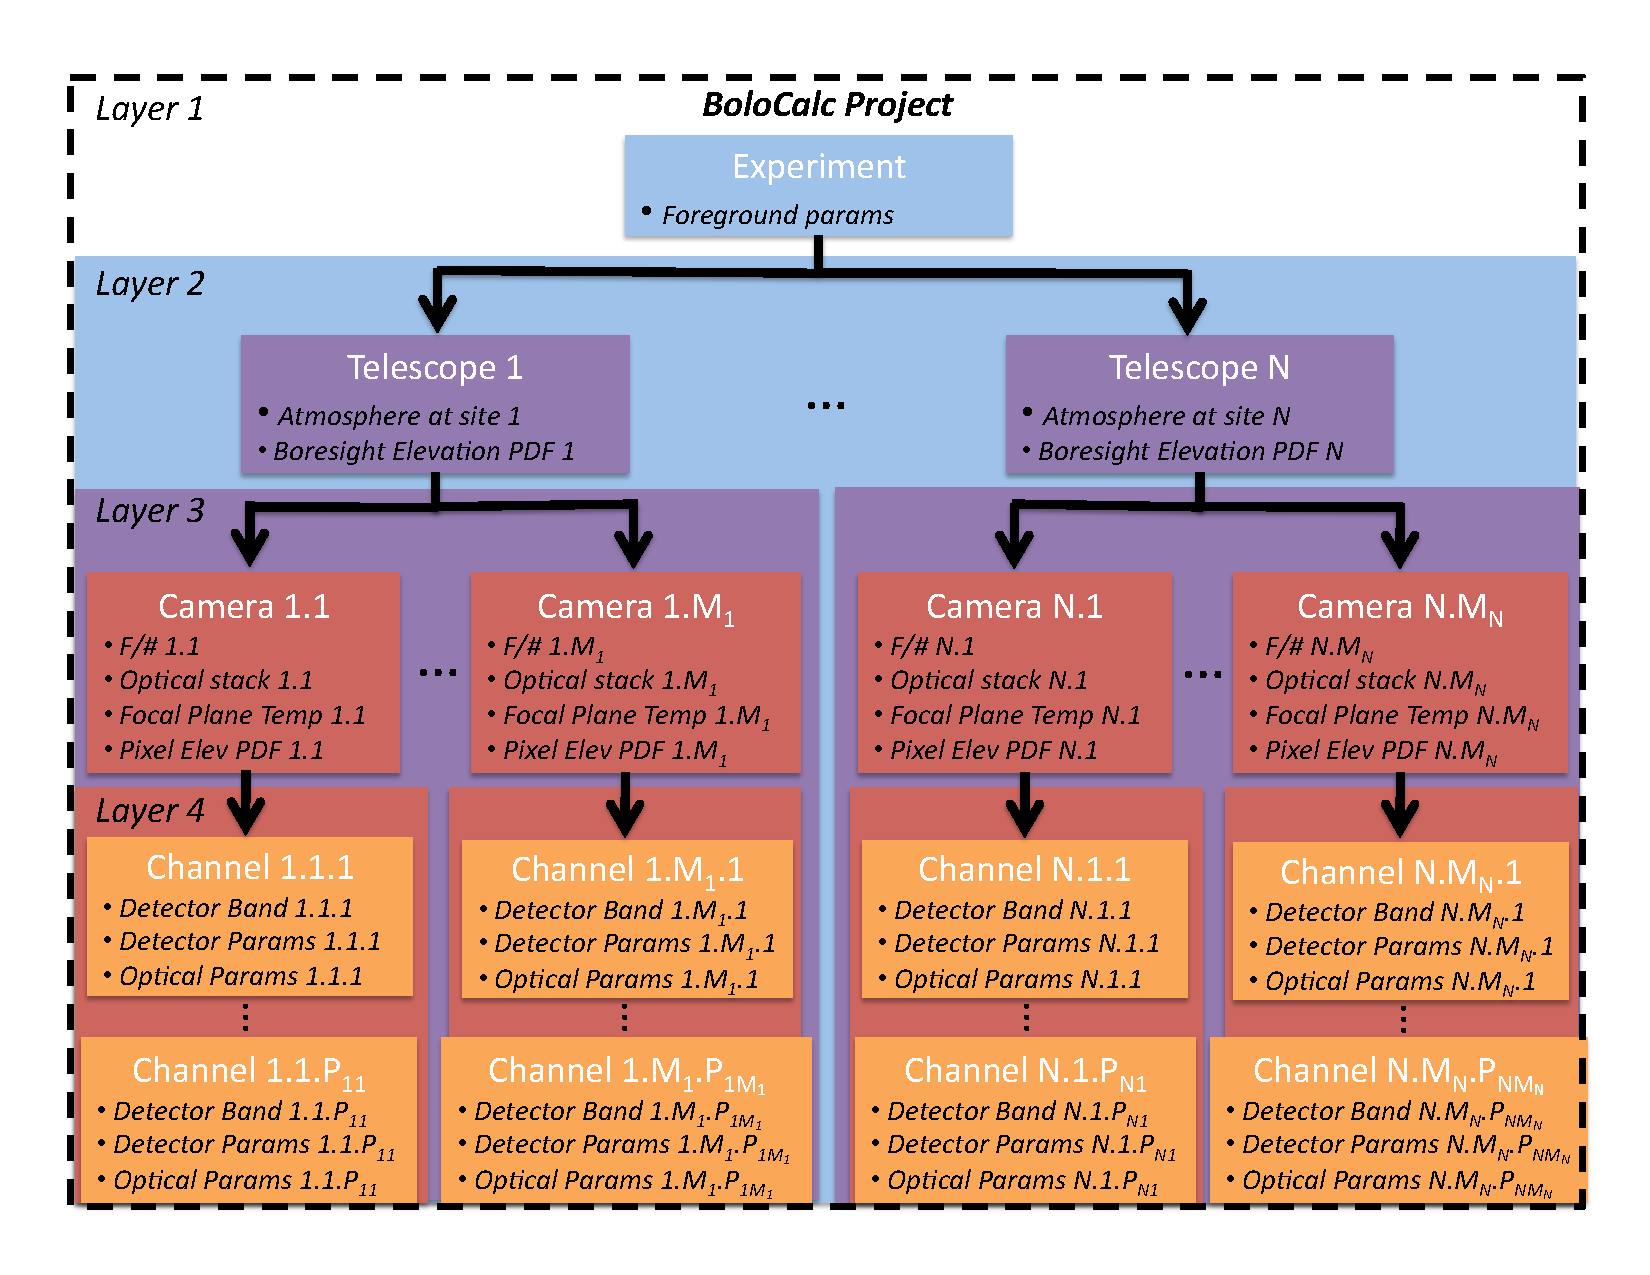
\includegraphics[trim={1cm, 0.8cm, 1.1cm, 1cm}, clip, width=1.00\textwidth]{OrgDiagram.pdf}
	\caption{Layout of a BoloCalc project. \label{fig:expstruct}}
\end{figure}

Each layer of an experiment has several parameters that define the input experiment. In this section, we go through them by input file.

%%%%%%%%%%%%%%%%%%%%%%%%%%%%%%%%%

\subsection{Directory Layout}

The experiment directory is meant to be easily generalizeable to various kinds of experiments and telescopes. Below is an overview of the file structure.

\begin{lstlisting}
	BoloCalc/Experiements/[Experiment Name]/[Experiment Design]
 	 |-- config
	 |    |--foregrounds.txt
	 |--Telescope 1/
	 |    |-- config/
	 |    |    |-- telescope.txt
	 |    |    |-- elevation.txt
	 |    |    |-- [Custom Atmospheric Profile] (optional)
	 |    |-- Camera 1/
	 |    |     |-- config/
	 |    |          |-- camera.txt
	 |    |          |-- channels.txt
	 |    |          |-- optics.txt
	 |    |          |-- elevation.txt
	 |    |          |-- Bands/
	 |    |	             |-- [Optic Band File 1] (optional)
	 |    |	             |-- [Optic Band File 2] (optional)
	 |    |	             |-- ...
	 |    |	             |-- [Detector Band File 1] (optional)
	 |    |	             |-- [Detector Band File 2] (optional)
	 |    |		    |-- ...
	 |    |-- Camera 2/
	 |    |-- ...
	 |-- Telescope 2/
	 |-- ...
\end{lstlisting}

As stated in Section \ref{sec:defexp}, an experiment definition has four layers:

\begin{enumerate}[noitemsep,topsep=0pt]
\item Experiment
\begin{itemize}[noitemsep,topsep=0pt]
	\item Composed of (multiple) telescopes
	\item All telescopes in a given experiment see the same galactic foregrounds
\end{itemize}
\item Telescopes
\begin{itemize}[noitemsep,topsep=0pt]
	\item Composed of (multiple) cameras
	\item All cameras in a given telescope see the same atmosphere
	\item All cameras in a given telescope have the same scan strategy 
\end{itemize}
\item Cameras
\begin{itemize}[noitemsep,topsep=0pt]
	\item Composed of (multiple) frequency channels
	\item All frequency channels in a given camera have the same camera parameters
	\item All frequency channels in a given camera see the same optical chain
\end{itemize}
\item Channels
\begin{itemize}[noitemsep,topsep=0pt]
	\item Each channel has independent detector and optical element parameters
\end{itemize}
\end{enumerate}

These layers allow telescopes to added to an experiment in an arbitrary location, each with arbitrary cameras, each with arbitrary frequency channels.

%%%%%%%%%%%%%%%%%%%%%%%%%%%%%%%%%

\subsection{Parameter Definitions}

All parameters in \texttt{BoloCalc} are defined with a central value and an error bar. Therefore, all parameter variation is assumed to have an underlying Gaussian distribution, and all parameters are assumed to be uncorrelated. 

Parameters defined \texttt{foregrounds.txt}, \texttt{telescope.txt}, \texttt{camera.txt}, and \texttt{channels.txt} have the following format:

\begin{lstlisting}
	Mean +/- Std Dev
\end{lstlisting}

The following formatting rules should be followed for the code to work robustly and the tables to render neatly:

\begin{enumerate}
	\item All central values and standard deviations should have five characters. For instance, \texttt{1.000} and \texttt{10.00} are valid, while \texttt{10.000} is not.
	\item All central values and standard deviations should be separated by  \texttt{ +/- }, noting the spaces on either side of the $+/-$ sign.
\end{enumerate}

Parameters defined in \texttt{optics.txt} are defined for multiple bands in multi-chroic cameras and therefore follow a different format:

\begin{lstlisting}
	[Mean for Band 1, Mean for Band 2, ...] +/- [Std Dev for Band 1, Std Dev for Band 2, ...]
\end{lstlisting}

In a similar way as with the single values, the following formatting rules should be followed for the code to work robustly and the tables to render neatly:

\begin{enumerate}
	\item All central values and standard deviations should have five characters. For instance, \texttt{1.000} and \texttt{10.00} are valid, while \texttt{10.000} is not.
	\item All arrays of central values and arrays of standard deviations should be separated by  \texttt{ +/- }, noting the spaces on either side of the $+/-$ sign
\end{enumerate}

%%%%%%%%%%%%%%%%%%%%%%%%%%%%%%%%%

\subsection{Experiment Parameters}

The experiment is comprised of an arbitrary set of telescopes, which are assumed to see the same the same celestial loading, including power from the CMB and galactic foregrounds.

%%%%%%%%%%%%%%%

\subsubsection{\texttt{foregrounds.txt}}

The below list overviews the parameters defined in \texttt{foregrounds.txt}, the file that defines the galaxy through which the telescope must observe the CMB. This galactic parameters will be the same for all telescopes.

\begin{itemize}[noitemsep,topsep=0pt]
	\item \textbf{Dust Temperature}
		\begin{itemize}[noitemsep,topsep=0pt]
		\item \textit{Description}: Dust modified blackbody temperature 
		\item \textit{Allowed Values}: Floating point value between (0.0, $+\infty$) K
		\item \textit{Default Value}: 19.70
		\end{itemize}
	\item \textbf{Dust Spec Index}
		\begin{itemize}[noitemsep,topsep=0pt]
		\item \textit{Description}: The spectral index of the dust modified blackbody spectrum
		\item \textit{Allowed Values}: Floating point value between ($-\infty$, $+\infty$)
		\item \textit{Default Value}: 1.50
		\end{itemize}
	\item \textbf{Dust Amplitude}
		\begin{itemize}[noitemsep,topsep=0pt]
		\item \textit{Description}: Amplitude of the dust modified blackbody spectrum 
		\item \textit{Allowed Values}: Floating point value between (0.0, $+\infty$)
		\item \textit{Default Value}: $2 \times 10^{-3}$
		\end{itemize}
	\item \textbf{Dust Scale Frequency}
		\begin{itemize}[noitemsep,topsep=0pt]
		\item \textit{Description}: Scale frequency for the dust modified blackbody spectrum
		\item \textit{Allowed Values}: Floating point value between (0.0, $+\infty$)
		\item \textit{Default Value}: 353.0 GHz
		\end{itemize}
	\item \textbf{Synchrotron Spec Index}
		\begin{itemize}[noitemsep,topsep=0pt]
		\item \textit{Description}: Spectral index of the synchrotron power law spectrum
		\item \textit{Allowed Values}: Floating point value between ($-\infty$, $+\infty$]
		\item \textit{Default Value}: $2 \times 10^{-3}$
		\end{itemize}
	\item \textbf{Synchrotron Amplitude}
		\begin{itemize}[noitemsep,topsep=0pt]
		\item \textit{Description}: Amplitude of the synchrotron power law spectrum
		\item \textit{Allowed Values}: Floating point value between (0.0, $+\infty$)
		\item \textit{Default Value}: $6 \times 10^{3}$
		\end{itemize}
\end{itemize}

%%%%%%%%%%%%%%%%%%%%%%%%%%%%%%%%%

\subsection{Telescope Parameters}
\label{sec:telparams}

In the following sections, we will overview the input parameters for each of the telescope input files.

%%%%%%%%%%%%%%%

\subsubsection{\texttt{telescope.txt}}
\label{sec:telescope}

The below list overviews the parameters defined in \texttt{telescope.txt}, the file that defines programmatic inputs to the telescope.

\begin{itemize}[noitemsep,topsep=0pt]
	\item \textbf{Site}
		\begin{itemize}[noitemsep,topsep=0pt]
		\item \textit{Description}: Site at which the telescope observes, which defines the atmospheric conditions. 
		\item \textit{Allowed Values}: Either ``Atacama'' or ``Pole''
		\item \textit{Default Value}: ``Atacama''
		\end{itemize}
	\item \textbf{Elevation}
		\begin{itemize}[noitemsep,topsep=0pt]
		\item \textit{Description}: Elevation at which the telescope observes. 
		\item \textit{Allowed Values}: [20.0, 90.0] deg above the horizon
		\item \textit{Default Value}: 50.0 deg
		\item If ``NA,'' the elevation distribution defined in \texttt{Telescope/config/elevation.txt}, will be assumed.
		\end{itemize}
	\item \textbf{PWV}
		\begin{itemize}[noitemsep,topsep=0pt]
		\item \textit{Description}: PWV of the atmosphere through which the telescope observes.
		\item \textit{Allowed Values}: [0.0, 8.0] mm
		\item \textit{Default Value}: 1.0 mm
		\item If ``NA,'' the PWV distribution defined in \texttt{Telescope/config/pwv.txt}, will be assumed.
		\end{itemize}
	\item \textbf{Observation Time}
		\begin{itemize}[noitemsep,topsep=0pt]
		\item \textit{Description}: How long this telescope will observe 
		\item \textit{Allowed Values}: Floating point value between (0.0, $+\infty$) years
		\item \textit{Default Value}: 3.0
		\end{itemize}
	\item \textbf{Sky Fraction}
		\begin{itemize}[noitemsep,topsep=0pt]
		\item \textit{Description}: What fraction of the sky this telescope will observe
		\item \textit{Allowed Values}: Floating point value between (0.0, 1.0]
		\item \textit{Default Value}: 0.7
		\end{itemize}
	\item \textbf{Observation Efficiency}
		\begin{itemize}[noitemsep,topsep=0pt]
		\item \textit{Description}: What fraction of the observation time will the telescope be actually observing 
		\item \textit{Allowed Values}: Floating point value between (0.0, 1.0]
		\item \textit{Default Value}: 0.8
		\end{itemize}
	\item \textbf{NET Margin}
		\begin{itemize}[noitemsep,topsep=0pt]
		\item \textit{Description}: Agnostic factor which multiplies the detector NETs for this telescope 
		\item \textit{Allowed Values}: Floating point value between (0.0, $+\infty$)
		\item \textit{Default Value}: 1.0
		\end{itemize}
\end{itemize}

%%%%%%%%%%%%%%%

\subsubsection{\texttt{elevation.txt}}
\label{sec:telelv}

\texttt{elevation.txt} is an optional file that defines the elevation probability distribution function (PDF), which is determined by the scan strategy of the telescope. The first column is the elevation above the horizon in degrees, and the second column is the fraction if time spent at that elevation. 

This file is only used if the parameter ``Elevation'' in \texttt{Telescope/config/elevation.txt} is defined to be ``NA'' (see Section \ref{sec:telescope} for more information about \texttt{telescope.txt}).

The probabilities should add up to one, and if they do not, the fraction will be determined by the provided probability divided by the sum of the provided probabilities.

Below is a made-up example for \texttt{elevation.txt}. Notice that each row is separated by a commented line of hyphens, while each column is separated by a vertical bar.

\begin{lstlisting}
	#*****Elevation Distribution******
	#
	Elevation     | Probability
	#---------------------------
	[deg]         | NA
	#---------------------------
	30.0          | 0.100
	#---------------------------
	40.0          | 0.100
	#---------------------------
	50.0          | 0.300
	#---------------------------
	60.0          | 0.400
	#---------------------------
	70.0          | 0.100
	#---------------------------
\end{lstlisting}

%%%%%%%%%%%%%%%

\subsubsection{\texttt{atm.txt}}

There is an option to override the code's handling of the atmosphere by providing a custom atmospheric profile. The atmosphere file must be in \texttt{[Telescope Name]/config/}, and the filename must have the form \texttt{atm\_[Elevation]deg\_[PWV]um.txt}. For example, a valid filename is \texttt{atm\_60deg\_1000um.txt}.

The atmosphere file should have four columns, delimited by white space:

\begin{enumerate}[noitemsep,topsep=0pt]
	\item Frequency [GHz]
	\item Optical Depth
	\item Planck Temperature [K]
	\item Transmission
\end{enumerate} 

\begin{lstlisting}
	| Frequency [GHz] | Optical Depth | Planck Temp [K] | Transmission |
\end{lstlisting}

Note that the temperature is in Planck units, not Rayleigh-Jeans. The passed frequency range in the atmosphere file needs to be large enough to cover the frequency bands observed by the telescope with at least a 15\% buffer on the bandwidths of the highest and lowest bands. For instance, if you want to know the atmospheric loading in a band from 240 to 300~GHz, your atmosphere file should have values that go up to at least 345~GHz.

Below is an example of an atmospheric profile generated using the AM simulation code and a configuration file designed using the 10-year MERRA dataset for the Chajnantor Observatory.

\begin{lstlisting}
	1.0000000e+01 3.664259e-03 3.589557e+00 9.963424e-01
	1.0020000e+01 3.667538e-03 3.590339e+00 9.963392e-01
	1.0040000e+01 3.671011e-03 3.591163e+00 9.963357e-01
	1.0060000e+01 3.674741e-03 3.592043e+00 9.963320e-01
	1.0080000e+01 3.678826e-03 3.593001e+00 9.963279e-01
	1.0100000e+01 3.683414e-03 3.594069e+00 9.963234e-01
	1.0120000e+01 3.688744e-03 3.595301e+00 9.963181e-01
	1.0140000e+01 3.695220e-03 3.596788e+00 9.963116e-01
	1.0160000e+01 3.703583e-03 3.598698e+00 9.963033e-01
	1.0180000e+01 3.715317e-03 3.601374e+00 9.962916e-01
	1.0200000e+01 3.733976e-03 3.605660e+00 9.962730e-01
	...
\end{lstlisting}

%%%%%%%%%%%%%%%%%%%%%%%%%%%%%%%%%

\subsection{Camera Parameters}

In the following sections, we will overview the input parameters for each of the camera input files.

%%%%%%%%%%%%%%%

\subsubsection{\texttt{camera.txt}}

\texttt{camera.txt} defines parameters that are the same for all frequency bands observed with this camera. The file must be located within \texttt{[Telescope Name]/[Camera Name]/config/}.

\begin{itemize}[noitemsep,topsep=0pt]
	\item \textbf{Boresight Elevation}
		\begin{itemize}[noitemsep,topsep=0pt]
		\item \textit{Description}: The elevation of the camera boresight with respect to the telescope boresight. 
		\item \textit{Allowed Values}: Floating point value between (-40.0, 40.0] deg
		\item \textit{Default Value}: 0.0 deg
		\end{itemize}
	\item \textbf{Optical Coupling}
		\begin{itemize}[noitemsep,topsep=0pt]
		\item \textit{Description}: How well the incident light on the focal plane couples to the pixel apertures 
		\item \textit{Allowed Values}: Floating point value between (0.0, 1.0]
		\item \textit{Default Value}: 1.0
		\end{itemize}
	\item \textbf{F-number}
		\begin{itemize}[noitemsep,topsep=0pt]
		\item \textit{Description}: The focal ratio at the focal plane
		\item \textit{Allowed Values}: Floating point value between (0.0, $+\infty$)
		\item \textit{Default Value}: 2.0
		\end{itemize}
	\item \textbf{Bath Temp}
		\begin{itemize}[noitemsep,topsep=0pt]
		\item \textit{Description}: The temperature of the focal plane 
		\item \textit{Allowed Values}: Floating point value between (0.0, $+\infty$) K
		\item \textit{Default Value}: 0.100
		\end{itemize}
\end{itemize}

%%%%%%%%%%%%%%%

\subsubsection{\texttt{elevation.txt}}

\texttt{elevation.txt} is an optional file that defines the elevation distribution with respect to the camera boresight of pixels on the focal plane. It has the exact same structure as the file \texttt{Telescope/config/elevation.txt}, which instead defines the scan strategy and is described in section \cite{sec:telelv}. The first column is the elevation above the horizon in degrees, and the second column is the fraction if time spent at that elevation. 

This file is only used if the parameter ``Elevation'' in \texttt{Telescope/config/elevation.txt} is defined to be ``NA'' (see Section \ref{sec:telescope} for more information about \texttt{telescope.txt}).

The probabilities should add up to one, and if they don not, the fraction will be determined by the provided probability divided by the sum of the provided probabilities.

Below is a made-up example of correct formatting for \texttt{elevation.txt}. Notice that each row is separated by a commented line of hyphens, while each colum is separated by a vertical bar.

\begin{lstlisting}
	#*****Elevation Distribution******
	#
	Elevation     | Probability
	#---------------------------
	[deg]         | NA
	#---------------------------
	30.0          | 0.100
	#---------------------------
	40.0          | 0.100
	#---------------------------
	50.0          | 0.300
	#---------------------------
	60.0          | 0.400
	#---------------------------
	70.0          | 0.100
	#---------------------------
\end{lstlisting}

%%%%%%%%%%%%%%%

\subsubsection{\texttt{channels.txt}}

\texttt{channels.txt} defines the parameters of the frequency bands and detectors that are observing in this camera. The file must be located within \texttt{[Telescope Name]/[Camera Name]/config/}.

\begin{itemize}[noitemsep,topsep=0pt]
	\item \textbf{Band ID}
		\begin{itemize}[noitemsep,topsep=0pt]
		\item \textit{Description}: The idenfitication number for this band 
		\item \textit{Allowed Values}: An integer value between [1, $+\infty$)
		\item \textit{Default Value}: 1
		\item Cannot have two bands with same Band ID on the same pixel
		\end{itemize}
	\item \textbf{Pixel ID}
		\begin{itemize}[noitemsep,topsep=0pt]
		\item \textit{Description}: The identification number for the pixel this band observes from
		\item \textit{Allowed Values}: An integer value between [1, $+\infty$)
		\item \textit{Default Value}: 1
		\end{itemize}
	\item \textbf{Band Center}
		\begin{itemize}[noitemsep,topsep=0pt]
		\item \textit{Description}: The central frequency for this band 
		\item \textit{Allowed Values}: A floating point value between (0.0, $+\infty$) GHz
		\item \textit{Default Value}: 145.0
		\end{itemize}
	\item \textbf{Fractional BW}
		\begin{itemize}[noitemsep,topsep=0pt]
		\item \textit{Description}: Fractional arithmetic bandwdith for this band 
		\item \textit{Allowed Values}: A floating point value between (0.0, 2.0]
		\item \textit{Default Value}: 0.276
		\end{itemize}
	\item \textbf{Pixel Size}
		\begin{itemize}[noitemsep,topsep=0pt]
		\item \textit{Description}: Size of the pixel via which this band is observing 
		\item \textit{Allowed Values}: A postive floating point value between (0.0, $+\infty$) mm
		\item \textit{Default Value}: 6.8
		\end{itemize}
	\item \textbf{Num Det per Wafer}
		\begin{itemize}[noitemsep,topsep=0pt]
		\item \textit{Description}: Number of detectors per wafer within this band
		\item \textit{Allowed Values}: An integer value between [1, $+\infty$)
		\item \textit{Default Value}: 542
		\end{itemize}
	\item \textbf{Num Waf per OT}
		\begin{itemize}[noitemsep,topsep=0pt]
		\item \textit{Description}: Number of wafers with this band per camera
		\item \textit{Allowed Values}: An integer value between [1, $+\infty$)
		\item \textit{Default Value}: 7
		\end{itemize}
	\item \textbf{Num OT}
		\begin{itemize}[noitemsep,topsep=0pt]
		\item \textit{Description}: Number of cameras in this telescope observing at this frequency 
		\item \textit{Allowed Values}: An integer value between [1, $+\infty$)
		\item \textit{Default Value}: 1
		\end{itemize}
	\item \textbf{Waist Factor}
		\begin{itemize}[noitemsep,topsep=0pt]
		\item \textit{Description}: The ratio of the gaussian beam waist coming from the pixel aperture to the pixel aperture diameter for this band 
		\item \textit{Allowed Values}: A floating point value between [2.0, +$\infty$) 
		\item \textit{Default Value}: 3.0
		\end{itemize}
	\item \textbf{Det Eff}
		\begin{itemize}[noitemsep,topsep=0pt]
		\item \textit{Description}: Efficiency of the detector from the entry point of the pixel aperture to the bolometer
		\item \textit{Allowed Values}: A floating point value between (0.0, 1.0]
		\item \textit{Default Value}: 0.700
		\end{itemize}
	\item \textbf{Psat}
		\begin{itemize}[noitemsep,topsep=0pt]
		\item \textit{Description}: Saturation power of the bolometer 
		\item \textit{Allowed Values}: A floating point value between (0.0, $+\infty$] pW
		\item \textit{Default Value}: ``NA''
		\item If ``NA,'' use ``Psat Factor'' to calculate ``Psat''
		\end{itemize}
	\item \textbf{Psat Factor}
		\begin{itemize}[noitemsep,topsep=0pt]
		\item \textit{Description}: Safety factor used to caculate saturation power from optical power
		\item \textit{Allowed Values}: A floating point value between (0.0, $+\infty$)
		\item \textit{Default Value}: 3.0
		\item If ``Psat'' is ``NA,'' calculate $P_{sat} = P_{opt} \times \mathrm{``Psat \; Factor''}$
		\end{itemize}
	\item \textbf{Carrier Index}
		\begin{itemize}[noitemsep,topsep=0pt]
		\item \textit{Description}: Thermal carrier index for bolometer leg conductivity 
		\item \textit{Allowed Values}: A floating point value between (0.0, $+\infty$)
		\item \textit{Default Value}: 2.7
		\end{itemize}
	\item \textbf{Tc}
		\begin{itemize}[noitemsep,topsep=0pt]
		\item \textit{Description}: Bolometer superconducting transition temperature
		\item \textit{Allowed Values}: A floating point value between (0.0, $+\infty$) K
		\item \textit{Default Value}: 0.159
		\item If ``NA,'' use ``Tc Fraction'' to calculate ``Tc''
		\end{itemize}
	\item \textbf{Tc Fraction}
		\begin{itemize}[noitemsep,topsep=0pt]
		\item \textit{Description}: Factor used to calculate transition temperature from the bath temperature 
		\item \textit{Allowed Values}: A floating point value between (1.0, $+\infty$)
		\item \textit{Default Value}: ``NA''
		\item If ``Tc'' is ``NA,'' calculate $T_{c} = T_{b} \times \mathrm{``Tc \; Fraction''}$
		\end{itemize}
	\item \textbf{Yield}
		\begin{itemize}[noitemsep,topsep=0pt]
		\item \textit{Description}: Fraction of deployed detectors that are observing. This is also commonly referred to as ``end-to-end'' yield. 
		\item \textit{Allowed Values}: A floating point value between (0.0, 1.0]
		\item \textit{Default Value}: 0.700
		\end{itemize}
	\item \textbf{SQUID NEI}
		\begin{itemize}[noitemsep,topsep=0pt]
		\item \textit{Description}: SQUID noise equivalent current 
		\item \textit{Allowed Values}: A floating point value between (0.0, $+\infty$) pA/$\sqrt{\mathrm{Hz}}$
		\item \textit{Default Value}: ``NA''
		\item If ``NA,'' ``Read Noise Frac'' is used to calculate readout noise
		\end{itemize}
	\item \textbf{Bolo Resistance}
		\begin{itemize}[noitemsep,topsep=0pt]
		\item \textit{Description}: Bolometer resistance 
		\item \textit{Allowed Values}: A floating point value between (0.0, $+\infty$) $\mathrm{\Omega}$
		\item \textit{Default Value}: ``NA''
		\item If ``NA,'' ``Read Noise Frac'' is used to calculate readout noise
		\end{itemize}
	\item \textbf{Read Noise Frac}
		\begin{itemize}[noitemsep,topsep=0pt]
		\item \textit{Description}: Fraction of the total NEP that is due to readout noise
		\item \textit{Allowed Values}: A floating point value between [0.0, $+\infty$) 
		\item \textit{Default Value}: 0.100
		\item If ``SQUID NEI'' or ``Bolo Resistance'' are ``NA,'' then calculate readout NEP as $NEP_{\mathrm{read}} = \sqrt{(1 + (\mathrm{``Read \; Noise \; Frac''}))^{2} - 1} \times \sqrt{NEP_{\mathrm{ph}}^{2} + NEP_{\mathrm{g}}^{2}}$. If ``NA,'' readout noise is zero.
		\end{itemize}
\end{itemize}

%%%%%%%%%%%%%%%

\subsubsection{\texttt{optics.txt}}

\texttt{optics.txt} defines the parameters the frequency bands and detectors that are observing in this camera. The file must be located within \texttt{[Telescope Name]/[Camera Name]/config/}.

\begin{itemize}[noitemsep,topsep=0pt]
	\item \textbf{Element}
		\begin{itemize}[noitemsep,topsep=0pt]
		\item \textit{Description}: Name of optical element
		\item \textit{Allowed Values}: Any string
		\item \textit{Default Value}: ``Element''
		\item ``Primary,'' ``Mirror,'' ``Aperture,'' and ``Stop'' trigger additional calculations and therefore must be used purposefully
		\end{itemize}
	\item \textbf{Temperature}
		\begin{itemize}[noitemsep,topsep=0pt]
		\item \textit{Description}: Temperature of the optical element
		\item \textit{Allowed Values}: An floating point value between (0.0, $+\infty$)
		\item \textit{Default Value}: 4.0
		\end{itemize}
	\item \textbf{Absorption}
		\begin{itemize}[noitemsep,topsep=0pt]
		\item \textit{Description}: Fractional power attenuation due to absorption within the optical element 
		\item \textit{Allowed Values}: A floating point value between [0.0, 1.0)
		\item \textit{Default Value}: 0.000
		\item If ``NA'' ...
			\begin{itemize}[noitemsep,topsep=0pt]
			\item If ``Mirror'' or ``Primary'' is in ``Element,'' ``Conductivity'' is used to calculate ohmic losses in the reflective optical element
			\item If ``Mirror'' or ``Primary'' is not in ``Element,'' ``Thickness,'' ``Index,'' and ``Loss Tangent'' are used to calculate dielectric loss in the refractive optical element
			\end{itemize}
		\end{itemize}
	\item \textbf{Reflection}
		\begin{itemize}[noitemsep,topsep=0pt]
		\item \textit{Description}: Fractional power lost due to reflection at the optical element 
		\item \textit{Allowed Values}: A floating point value between [0.0, 1.0)
		\item \textit{Default Value}: 0.000
		\item If ``NA'' ...
			\begin{itemize}[noitemsep,topsep=0pt]
			\item If ``Mirror'' or ``Primary'' is in ``Element,'' ``Surface Rough'' is used to reflection loss in the reflective optic
			\item If ``Mirror'' or ``Primary'' is not in ``Element,'' relfection is assumed be zero
			\end{itemize}
		\end{itemize}
	\item \textbf{Thickness}
		\begin{itemize}[noitemsep,topsep=0pt]
		\item \textit{Description}: Thickness of the optical element
		\item \textit{Allowed Values}: A floating point value between (0.0, $+\infty$) mm
		\item \textit{Default Value}: ``NA''
		\item If ``Absorption'' is ``NA,'' ... 
			\begin{itemize}[noitemsep,topsep=0pt]
			\item If ``Thickness'' is ``NA,'' absorption is assumed be zero
			\item If ``Thickness'' is not ``NA,'' 
				\begin{itemize}[noitemsep,topsep=0pt]
				\item If ``Mirror'' or ``Primary'' is in ``Element,'' this parameter is ignored
				\item If ``Mirror'' or ``Primary'' is not in ``Element,'' this parameter is used to calculate dielectric loss in the refractive optic
				\end{itemize}
			\end{itemize}
		\item If ``Absorption'' is not ``NA,'' this parameter is ignored
		\end{itemize}
	\item \textbf{Index}
		\begin{itemize}[noitemsep,topsep=0pt]
		\item \textit{Description}: Index of refraction of the optical elemet 
		\item \textit{Allowed Values}: A floating point value between [1.0, $+\infty$)
		\item \textit{Default Value}: ``NA''
		\item If ``Absorption'' is ``NA,'' ... 
			\begin{itemize}[noitemsep,topsep=0pt]
			\item If ``Index'' is ``NA,'' absorption is assumed be zero
			\item If ``Index'' is not ``NA,'' 
				\begin{itemize}[noitemsep,topsep=0pt]
				\item If ``Mirror'' or ``Primary'' is in ``Element,'' this parameter is ignored
				\item If ``Mirror'' or ``Primary'' is not in ``Element,'' this parameter is used to calculate dielectric loss in the refractive optic
				\end{itemize}
			\end{itemize}
		\item If ``Absorption'' is not ``NA,'' this parameter is ignored
		\end{itemize}
	\item \textbf{Loss Tangent}
		\begin{itemize}[noitemsep,topsep=0pt]
		\item \textit{Description}: Loss tangent of the optical element
		\item \textit{Allowed Values}: A floating point value between [0.0, $+\infty$)
		\item \textit{Default Value}: ``NA''
		\item If ``Absorption'' is ``NA,'' ... 
			\begin{itemize}[noitemsep,topsep=0pt]
			\item If ``Loss Tangent'' is ``NA,'' absorption is assumed be zero
			\item If ``Loss Tangent'' is not ``NA,'' 
				\begin{itemize}
				\item If ``Mirror'' or ``Primary'' is in ``Element,'' this parameter is ignored
				\item If ``Mirror'' or ``Primary'' is not in ``Element,'' this parameter is used to calculate dielectric loss in the refractive optic
				\end{itemize}
			\end{itemize}
		\item If ``Absorption'' is not ``NA,'' this parameter is ignored
		\end{itemize}
	\item \textbf{Conductivity}
		\begin{itemize}[noitemsep,topsep=0pt]
		\item \textit{Description}: Electrical conductivity of the optical element 
		\item \textit{Allowed Values}: A floating point value between (0.0, $+\infty$)
		\item \textit{Default Value}: ``NA''
		\item If ``Absorption'' is ``NA,'' ... 
			\begin{itemize}[noitemsep,topsep=0pt]
			\item If ``Conductivity'' is ``NA,'' absorption is assumed be zero
			\item If ``Conductivity'' is not ``NA,'' 
				\begin{itemize}
				\item If ``Mirror'' or ``Primary'' is in ``Element,'' this parameter is used to calculate dielectric loss in the reflective optic
				\item If ``Mirror'' or ``Primary'' is not in ``Element,'' this parameter is ignored
				\end{itemize}
			\end{itemize}
		\item If ``Absorption'' is not ``NA,'' this parameter is ignored		
		\end{itemize}
	\item \textbf{Surface Rough}
		\begin{itemize}[noitemsep,topsep=0pt]
		\item \textit{Description}: Surface roughness of the optical element 
		\item \textit{Allowed Values}: A floating point value between [0.0, +$\infty$) 
		\item \textit{Default Value}: ``NA''
		\item If ``Reflection'' is ``NA,'' ... 
			\begin{itemize}[noitemsep,topsep=0pt]
			\item If ``Surface Rough'' is ``NA,'' absorption is assumed be zero
			\item If ``Surface Rough'' is not ``NA,'' 
				\begin{itemize}[noitemsep,topsep=0pt]
				\item If ``Mirror'' or ``Primary'' is in ``Element,'' this parameter is used to calculate the reflection loss due to Ruze Scattering in the reflective optic
				\item If ``Mirror'' or ``Primary'' is not in ``Element,'' this parameter is ignored
				\end{itemize}
			\end{itemize}
		\item If ``Reflection'' is not ``NA,'' this parameter is ignored
		\end{itemize}
	\item \textbf{Spillover}
		\begin{itemize}[noitemsep,topsep=0pt]
		\item \textit{Description}: Fractional power that spills over the optical element
		\item \textit{Allowed Values}: A floating point value between [0.0, 1.0)
		\item \textit{Default Value}: ``NA''
		\item If this parameter is ``NA,'' spillover is assumed be zero
		\end{itemize}
	\item \textbf{Spillover Temp}
		\begin{itemize}[noitemsep,topsep=0pt]
		\item \textit{Description}: The effective temperature that the spilled power lands on 
		\item \textit{Allowed Values}: A floating point value between [0.0, $+\infty$)
		\item \textit{Default Value}: ``NA''
		\item If ``NA,'' spillover is assumed to land at ``Temperature,'' the temperature of the element itself
		\end{itemize}
	\item \textbf{Scatter Frac}
		\begin{itemize}[noitemsep,topsep=0pt]
		\item \textit{Description}: Fraction of the reflected power that is scatterd out of the propogation mode
		\item \textit{Allowed Values}: A floating point value between [0.0, 1.0]
		\item \textit{Default Value}: ``NA''
		\item If ``NA,'' scattering is assumed to be zero.
		\end{itemize}
	\item \textbf{Scatter Temp}
		\begin{itemize}[noitemsep,topsep=0pt]
		\item \textit{Description}: The effective temperature that the scattered power lands on 
		\item \textit{Allowed Values}: A floating point value between [0.0, $+\infty$)
		\item \textit{Default Value}: ``NA''
		\item If ``NA,'' scattered power is assumed to land at ``Temperature,'' the temperature of the optical element itself
		\end{itemize}
\end{itemize}

%%%%%%%%%%%%%%%%%%%%%%%%%%%%%%%%%

\subsection{Custom Bands}

By default, \texttt{BoloCalc} assumes top hat bands for all detectors and optical elements, whose height is determined soley by the mean and standard deviation of the end-to-end optical efficiency. However, custom bands can be input for any optical element.

The general file format for all band files is the same:

\begin{lstlisting}
	| Frequency [GHz] | Mean Efficiency | Standard Deviation (optional) |
\end{lstlisting}

Each column is separated by a vertical bar, and the final column, which contains the error bars, can be omitted. If only two columns are present, all stand deviations are assumed to be zero.

An example of a made-up detector bandpass text file, which is space-delimited, is shown below:

\begin{lstlisting}
	70.     0.000   0.000
	75.     0.500   0.100
	80.     0.700   0.100
	85.     0.650   0.100
	90.     0.700   0.100
	100.    0.800   0.100
	105.    0.600   0.100
	110.    0.700   0.100
	115.    0.500   0.100
	120.    0.000   0.000
\end{lstlisting}

%%%%%%%%%%%%%%%

\subsubsection{Detectors}

Detector band files are stored in

\begin{lstlisting}
	[Telescope Name]/[Camera Name]/config/Bands/Detectors/
\end{lstlisting}

The band is identified using its filename, which must have the format \texttt{[Camera Name][Band ID].txt} for text files, or \texttt{[Camera Name][Band ID].csv} for comma-separated value files; both file formats work equally well. For example, to load a text file for a camera named ``MF'' (in the directory \texttt{[Telescope Name]/MF/} and a Band ID ``1,'' the file name should be \texttt{MF1.txt}. Note that for a multi-chroic camera, there should be multiple band files, one for each frequency channel.

%%%%%%%%%%%%%%%

\subsubsection{Optics}

Optics band files are stored in

\begin{lstlisting}
	[Telescope Name]/[Camera Name]/config/Bands/Detectors/Optics/
\end{lstlisting}

The band is identified using its filename, which must have the format \texttt{[Optical Element Name].txt} for text files, or \texttt{[Optical Element Name].csv} for comma-separated value files; both file formats work equally well. For example, to load a text file for an optical element named ``Lens1,'' the file name should be \texttt{Lens1.txt}. Note that there is only one band file for optical elements, even in multi-chroic cameras, as all detectors are all frequencies see the same bandpass. Also note that you can apply the same band to multiple optical elements by duplicating matching names in \texttt{optics.txt}.

%%%%%%%%%%%%%%%%%%%%%%%%%%%%%%%%%%%%%%%%%%%%%%%%%%%%%%%%%%%%%%%%%%%%%%

\section{Output Files}

Running \texttt{mappingSpeed.py} generates several output files, which quantify the performance of the simulated experiment. Note that all examples in this document assume the Simons Observatory V3 configutation with no error bars for all parameters, with all observations at 60 deg elevation and 1 mm PWV.

%%%%%%%%%%%%%%%%%%%%%%%%%%%%%%%%%

\subsection{Sensitivity Tables}

\texttt{BoloCalc} produces tables of outputs related to the white noise performance of the instrument. All sensitivity tables are in files named \texttt{sensitivity.txt}, and there are multiple tables generated at multiple directory tree levels, describing the performance of the camera, telescope, and entire experiment.

%%%%%%%%%%%%%%%

\subsubsection{\texttt{Experiment/sensitivity.txt}}

This file lists the following parameters:

\begin{itemize}[noitemsep,topsep=0pt]
	\item \texttt{Chan}
		\begin{itemize}[noitemsep,topsep=0pt]
		\item Frequency channel name \texttt{[Camera Name][Band ID]}
		\end{itemize}
	\item \texttt{Frequency}
		\begin{itemize}[noitemsep,topsep=0pt]
		\item Central frequency of the frequency channel
		\end{itemize}
	\item \texttt{Frac Bandwidth} 
		\begin{itemize}[noitemsep,topsep=0pt]
		\item Fractional bandwidth of frequency channel
		\end{itemize}
	\item \texttt{Num Det}
		\begin{itemize}[noitemsep,topsep=0pt]
		\item Total number of detectors deployed in this frequency channel, combined for all telescopes within the experiment
		\end{itemize}
	\item \texttt{Array NET}
		\begin{itemize}[noitemsep,topsep=0pt]
		\item Aarray-averaged noise equivalent temperature of this frequency channel, combined for all telescopes within the experiment
		\end{itemize}
	\item \texttt{Mapping Speed}
		\begin{itemize}[noitemsep,topsep=0pt]	
		\item Mapping speed of this frequency channel, combined for all telescopes within the experiment
		\end{itemize}
	\item \texttt{Map Depth}
		\begin{itemize}[noitemsep,topsep=0pt]
		\item Map depth achieved by this frequency channel, combined for all telescopes within the experiment
		\end{itemize}
\end{itemize}
Note that if identical bands are shared between telescopes, the detectors are combined in this table, with the combined Array NET of that band is found by taking the inverse-variance average of the duplicated bands.

Below is an example of \texttt{sensitivity.txt} at the Experiment directory level:

\begin{figure}[h!]
	\centering
	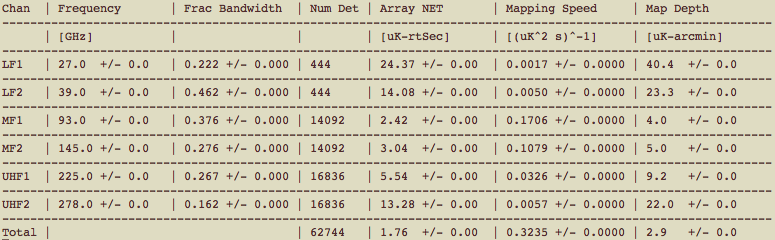
\includegraphics[width=1.0\textwidth]{Experiment_sensEx}
	\caption{Simons Observatory V3 experiment sensitivity, which combines the NETs from the Large Aperture Telescope and the Small Aperture Telescope. Both telescopes share wafers, and therefore have duplicates of each frequency band. The NETs are inverse-variace averaged in this sensitivity table for the entire experiment. \label{expSens}}
\end{figure}

%%%%%%%%%%%%%%%

\subsubsection{\texttt{Experiment/Telescope/sensitivity.txt}}

This file lists

\begin{itemize}[noitemsep,topsep=0pt]
	\item \texttt{Chan}
		\begin{itemize}[noitemsep,topsep=0pt]
		\item Frequency channel name \texttt{[Camera Name][Band ID]}
		\end{itemize}
	\item \texttt{Frequency}
		\begin{itemize}[noitemsep,topsep=0pt]
		\item Central frequency of the frequency channel
		\end{itemize}
	\item \texttt{Frac Bandwidth} 
		\begin{itemize}[noitemsep,topsep=0pt]
		\item Fractional bandwidth of frequency channel
		\end{itemize}
	\item \texttt{Num Det}
		\begin{itemize}[noitemsep,topsep=0pt]
		\item Total number of detectors deployed in this frequency channel, combined for all cameras within the telescope
		\end{itemize}
	\item \texttt{Array NET}
		\begin{itemize}[noitemsep,topsep=0pt]
		\item Aarray-averaged noise equivalent temperature of this frequency channel, combined for all cameras within the telescope
		\end{itemize}
	\item \texttt{Mapping Speed}
		\begin{itemize}[noitemsep,topsep=0pt]	
		\item Mapping speed of this frequency channel, combined for all cameras within the telescope
		\end{itemize}
	\item \texttt{Map Depth}
		\begin{itemize}[noitemsep,topsep=0pt]
		\item Map depth achieved by this frequency channel, combined for all cameras within the telescope
		\end{itemize}
\end{itemize}
Note that if identical bands are shared between cameras, the detectors are combined in this table, with the combined Array NET of that band is found by taking the inverse-variance average of the duplicated bands.

Below is an example of \texttt{sensitivity.txt} at the Telescope directory level:

\begin{figure}[h!]
	\centering
	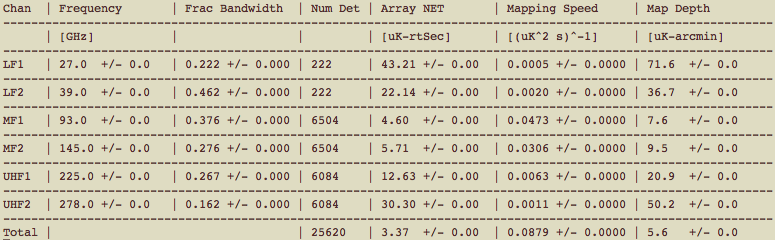
\includegraphics[width=1.0\textwidth]{Telescope_sensEx}
	\caption{Simons Observatory V3 Large Aperture Telescope sensitivity, which combines the NETs from the LF, MF, and UHF cameras. \label{telSens}}
\end{figure}

%%%%%%%%%%%%%%%

\subsubsection{\texttt{Experiment/Telescope/Camera/sensitivity.txt}}

This file lists

\begin{itemize}[noitemsep,topsep=0pt]
	\item \texttt{Chan}
		\begin{itemize}[noitemsep,topsep=0pt]
		\item Frequency channel name \texttt{[Camera Name][Band ID]}
		\end{itemize}
	\item \texttt{Frequency}
		\begin{itemize}[noitemsep,topsep=0pt]
		\item Central frequency of the frequency channel
		\end{itemize}
	\item \texttt{Frac Bandwidth} 
		\begin{itemize}[noitemsep,topsep=0pt]
		\item Fractional bandwidth of frequency channel
		\end{itemize}
	\item \texttt{Num Det}
		\begin{itemize}[noitemsep,topsep=0pt]
		\item Total number of detectors deployed in this frequency channel, combined for all cameras within the telescope
		\end{itemize}
		\item \texttt{Chan}
		\begin{itemize}[noitemsep,topsep=0pt]
		\item Frequency channel name \texttt{[Camera Name][Band ID]}
		\end{itemize}
	\item \texttt{Lyot Efficiency}
		\begin{itemize}[noitemsep,topsep=0pt]
		\item Lyot stop spillover efficiency of the frequency channel
		\end{itemize}
	\item \texttt{Optical Power} 
		\begin{itemize}[noitemsep,topsep=0pt]
		\item Total optical power on detectors within this frequency channel
		\end{itemize}
	\item \texttt{Photon NEP}
		\begin{itemize}[noitemsep,topsep=0pt]
		\item Noise-equivalent power due to photon noise for detectors within this frequency channel
		\end{itemize}
	\item \texttt{Bolometer NEP}
		\begin{itemize}[noitemsep,topsep=0pt]
		\item Noise-equivalent power due to bolometer thermal carrier noise for detectors within this frequency channel
		\end{itemize}
	\item \texttt{Detector NEP}
		\begin{itemize}[noitemsep,topsep=0pt]
		\item Total noise-equivalent power due to the combinatin of photon, thermal carrier, and readout noise for detectors within this frequency channel
		\end{itemize}
	\item \texttt{Detector NET} 
		\begin{itemize}[noitemsep,topsep=0pt]
		\item Per-detector noise-equivalent temperature for detectors within this channel
		\end{itemize}
	\item \texttt{Array NET}
		\begin{itemize}[noitemsep,topsep=0pt]
		\item Aarray-averaged noise equivalent temperature of this frequency channel
		\end{itemize}
	\item \texttt{Mapping Speed}
		\begin{itemize}[noitemsep,topsep=0pt]	
		\item Mapping speed of this frequency channel
		\end{itemize}
	\item \texttt{Map Depth}
		\begin{itemize}[noitemsep,topsep=0pt]
		\item Map depth achieved by this frequency channel
		\end{itemize}
\end{itemize}
for every frequency channel in the provided camera.

Below is an example of \texttt{sensitivity.txt} at the Camera directory level:

\begin{figure}[h!]
	\centering
	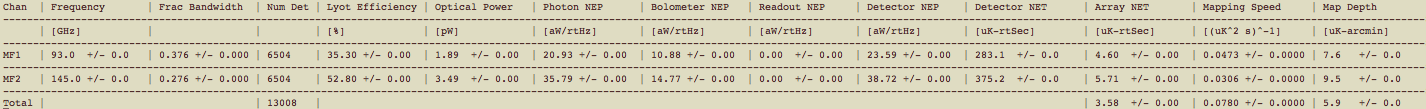
\includegraphics[width=1.0\textwidth]{Camera_sensEx}
	\caption{Simons Observatory V3 Large Aperture Telescope MF Camera sensitivity. \label{camSens}}
\end{figure}

%%%%%%%%%%%%%%%%%%%%%%%%%%%%%%%%%

\subsection{Optical Power Table}

\texttt{BoloCalc} also outputs tables of optical powers, including the the following information in columns:

\begin{itemize}[noitemsep,topsep=0pt]
	\item \texttt{Element}
		\begin{itemize}[noitemsep,topsep=0pt]
		\item Name of optical element, as defined within \texttt{optics.txt} for this camera
		\end{itemize}
	\item \texttt{Power from Sky}
		\begin{itemize}[noitemsep,topsep=0pt]
		\item Power incident on this optical element from the sky side
		\end{itemize}
	\item \texttt{Power to Detect}
		\begin{itemize}[noitemsep,topsep=0pt]
		\item Power emitted from this optical element which is seen by the detector
		\end{itemize}
	\item \texttt{Cumulative Eff}
		\begin{itemize}[noitemsep,topsep=0pt]
		\item Cumulative Efficiency between this optical emenet and the detector
		\end{itemize}
\end{itemize}

%%%%%%%%%%%%%%%

\subsubsection{\texttt{Experiment/Telescope/Camera/opticalPower.txt}}

Optical powers are listed for each channel in the camera, formatted as one table per frequency. Below is an example for the V3 Large Aperture Telescope Mid-Frequency camera.

\begin{figure}[h!]
	\centering
	\begin{subfigure}{0.49\linewidth}
		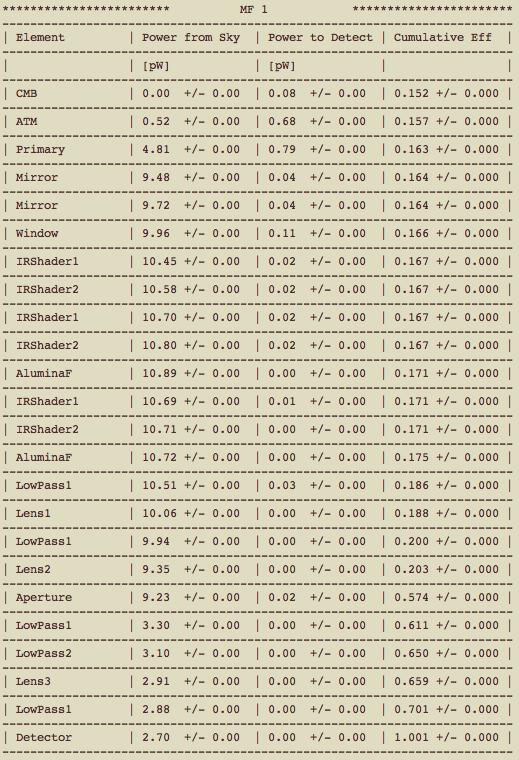
\includegraphics[width=1.0\linewidth]{Camera_optPowEx_1}
	\end{subfigure}
	\begin{subfigure}{0.49\linewidth}
		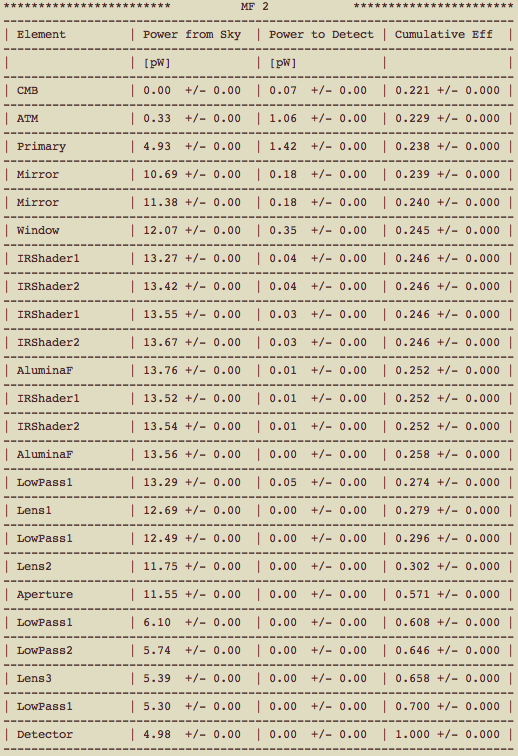
\includegraphics[width=1.0\linewidth]{Camera_optPowEx_2}
	\end{subfigure}
	\caption{Simons Observatory V3 Large Aperture Telescope Mid-Frequency camera optical power tables. Each table is labeled by ``[camera name] + [band name].'' \label{expSens}}
\end{figure}

%%%%%%%%%%%%%%%%%%%%%%%%%%%%%%%%%%%%%%%%%%%%%%%%%%%%%%%%%%%%%%%%%%%%%%

\section{Monte Carlo Simulation}

The Monte Carlo (MC) simulation iterates using a nest of the following structure:

\begin{itemize}[noitemsep,topsep=0pt]
	\item $N_{\mathrm{exp}}$ Experiment realizations
		\begin{itemize}[noitemsep,topsep=0pt]
		\item $N_{\mathrm{obs}}$ Observations per experiment realization
			\begin{itemize}[noitemsep,topsep=0pt]
			\item $N_{\mathrm{det}}$ Detector realizations per observation
			\end{itemize}
		\end{itemize}
\end{itemize}
	
The number of iterations performed at each level of the MC is determined by parameters in \texttt{BoloCalc/config/mappingSpeed\_params.txt}:

\begin{itemize}[noitemsep,topsep=0pt]
	\item $N_{\mathrm{exp}}$ = \texttt{Experiments}
	\item $N_{\mathrm{obs}}$ = \texttt{Observations}
	\item $N_{\mathrm{det}}$ = \texttt{Detectors}
\end{itemize}

If any of these parameters are set to one, then the mean value is taken for the parameters that vary with the experiment realization, observation, or detector realization, respectively. 

Below is a list of parameters that vary with each layer of the MC tree:

\begin{itemize}[noitemsep,topsep=0pt]
	\item \textbf{Experiment Realizations}
		\begin{itemize}[noitemsep,topsep=0pt]
		\item All parameters in \texttt{foregrounds.txt}
		\item All parameters in each  \texttt{telescope.txt} file
		\item All parameters in each \texttt{camera.txt} file
		\item All parameters in each \texttt{optics.txt} file
		\item Within all \texttt{channels.txt} files:
			\begin{itemize}[noitemsep,topsep=0pt]
			\item \texttt{Pixel Size}
			\item \texttt{Waist Factor}
			\item \texttt{Yield}
			\end{itemize}
		\end{itemize}
		\item All bands defined by files in \texttt{config/Bands/Optics/}
	\item \textbf{Observations}
		\begin{itemize}[noitemsep,topsep=0pt]
		\item PWV
		\item Elevation
		\end{itemize}
	\item \textbf{Detector Realizations}
		\begin{itemize}[noitemsep,topsep=0pt]
		\item Within all \texttt{channels.txt} files:
			\begin{itemize}[noitemsep,topsep=0pt]
			\item \texttt{Band Center}
			\item \texttt{Fractional BW}
			\item \texttt{Det Eff}
			\item \texttt{Psat}
			\item \texttt{Psat Factor}
			\item \texttt{Carrier Index}
			\item \texttt{Tc}
			\item \texttt{Tc Fraction}
			\item \texttt{SQUID NEI}
			\item \texttt{Bolo Resistance}
			\item \texttt{Read Noise Frac}
			\end{itemize}
		\item All bands defined by files in \texttt{config/Bands/Detectors/}
		\end{itemize}
\end{itemize}
		
\end{document}

%%%%%%%%%%%%%
%%%%% END %%%%%
%%%%%%%%%%%%%

%%%%%%%%%%%%%%%%%%%%%%%%%%%%%%%%%%%%%%%%%%%%%%%%%%%%%%%%%%%%%%%%%%%%%%

\section{Noise Calculation}

This section details the mapping speed calculation given the range of possible inputs described in previous sections. 

%%%%%%%%%%%%%%%%%%%%%%%%%%%%%%%%%

\subsection{Optical Power}

Optical power is calculated via

\begin{equation}
	P_{opt} = \int_{\nu_{1}}^{\nu_{2}} \; \Big[ \sum_{i = 0}^{N_{elem}}  P_{i} (T_{i}, T_{r;i}, \nu) \Big] \, \mathrm{d} \nu
	\label{eq:pOpt}
\end{equation}

where the summation runs over the optical elements from the sky towards the detector, and where $\nu_{1}$ and $\nu_{2}$ are the edges of the band in question. In Equation \ref{eq:pOpt}, I've defined 

\begin{equation}
	P_{i} (T_{i}, T_{r;i}, \nu) = E_{i} (\nu) \, S (T_{i}, \nu) + R_{i} (\nu) \, S (T_{r;i}, \nu)
	\label{eq:poptIntegrand}
\end{equation}

where $T_{i}$ is the temperature of optical element $i$, $T_{r;i}$ is the temperature that element $i$ reflects to, and $S(T, \nu)$ is the power spectrum as a function of frequency $\nu$ emitted from a blackbody at temperature $T$ onto a diffraction-limited aperture.

\begin{equation}
	S (T, \nu) = \frac{h \, \nu}{e^{\frac{h \nu}{k_{B} \, T}} - 1}
	\label{eq:powIntegrand}
\end{equation}

In Equation \ref{eq:poptIntegrand}, I've defined 

\begin{equation}
	E_{i} = \Big[ \prod_{j = i+1}^{N_{elem}} \, \eta_{j} (\nu) \Big] \, \epsilon_{i} (\nu)
	\label{eq:effEmiss}
\end{equation}

which is the effective emissivity due to absorption: $\epsilon_{i}$ is the dielectric emissivity of element $i$, and $\Big( \prod_{j = i+1}^{N_{elem}} \, \eta_{j} \Big)$ represents the cumulative efficiency of everything detector-side of element $i$. I've also defined 

\begin{equation}
	R_{i} = \Big[ \prod_{j = i+1}^{N_{elem}} \, \eta_{j} (\nu) \Big] \, r_{i} (\nu)
	\label{eq:reflEffEmiss}
\end{equation}

which is the effective emissivity due to reflection: $r_{i}$ is the reflectivity of element $i$, and $\Big( \prod_{j = i+1}^{N_{elem}} \, \eta_{j} \Big)$ represents the cumulative efficiency of everything detector-side of element $i$.

%%%%%%%%%%%%%%%%%%%%%%%%%%%%%%%%%

\subsection{Photon NEP}

We use the following equation to calculate the photon noise equivalent power (NEP)

\begin{equation}
	\mathrm{NEP_{ph}} = \sqrt{\int_{\nu_{1}}^{\nu_{2}} \, [ \, 2 h \nu \sum_{i}^{N_\mathrm{elem}}  P_{i} (T_{i}, T_{r;i}, \nu) + 2 \, (\sum_{i}^{N_\mathrm{elem}}  P_{i} (T_{i}, T_{r;i}, \nu))^{2} \, ] \mathrm{d}\nu}
\end{equation}


where $P_{i}$ is defined in Equation \ref{eq:poptIntegrand}. Notice that we assume 100\% photon bunching and that we integrate over the bunching cross terms.

%%%%%%%%%%%%%%%%%%%%%%%%%%%%%%%%%

\subsection{Thermal Carrier NEP}

We use the following equation to calculate thermal carrier noise inherent to the bolometer power dissipation

\begin{equation}
	\mathrm{NEP_{g}} = \sqrt{4 k_{B} P_{oper} T_{b} \frac{(n+1)^{2}}{2n + 3} \frac{(T_{c} / T_{b})^{2n + 3} - 1}{[(T_{c} / T_{b})^{n+1} - 1]^{2}}}
\end{equation}

where $T_{c} = 0.171$ K is the critical temperature, $T_{b} = 0.100$ K is the bath temperature, $n = 3$ because the thermal carrier is the phonon, and bolometer operation power is calculated as 

\begin{equation}
	P_{oper} = 2.5 \, P_{opt}
\end{equation}

%%%%%%%%%%%%%%%%%%%%%%%%%%%%%%%%%

\subsection{Readout NEP}

We mandate that the total NEP for each detector be low enough such that we can meet our $\sigma(r=0)$ requirement. Therefore, $NEP_{\mathrm{det}}$ is essentially fixed by the cosmology. To meet this requirement, we float the readout NEP, assuming that we can suppress it with more flexibility than the phton and bolometer noises. 

Hence, readout noise is calculated as 

\begin{equation}
	\mathrm{NEP_{read}} = \sqrt{\mathrm{NEP_{det}^{2} - NEP_{g}^{2} + NEP_{read}^{2}}}
\end{equation}

%%%%%%%%%%%%%%%%%%%%%%%%%%%%%%%%%

\subsection{Detector NEP}

We find the total detector noise by taking the quadrature sum of the photon, thermal, and readout NEP values

\begin{equation}
	\mathrm{NEP_{det}} = \sqrt{\mathrm{NEP_{ph}^{2} + NEP_{g}^{2} + NEP_{read}^{2}}}
\end{equation}

%%%%%%%%%%%%%%%%%%%%%%%%%%%%%%%%%

\subsection{Detector NET}

We calculate the noise equivalent temperature (NET) of a detector as kamThesis

\begin{equation}
	\mathrm{NET_{det}} = \frac{\mathrm{NEP_{det}}}{\sqrt{2} \, (\mathrm{dP/dT_{CMB}})}
\end{equation}

where we have defined the conversion factor from power to CMB temperature units as \cite{kamThesis}

\begin{equation}
	\mathrm{dP/dT_{CMB}} = \int_{\nu_1}^{\nu_{2}} \Big[ \, \frac{\eta}{k_{B}} \Big(\frac{h \nu}{T_{CMB} (e^{h \nu / k_{B} T_{CMB}} - 1)} \Big)^{2} \, e^{h \nu / k_{B} T_{CMB}} \, \Big] \mathrm{d}{\nu}
\end{equation}

where again, $\nu_{1}$ and $\nu_{2}$ are the edges of the band. Note that the $\sqrt{2}$ enters because NEP is defined in terms of $1/\sqrt{Hz}$ and NET is defined in terms of $\sqrt{sec}$.

%%%%%%%%%%%%%%%%%%%%%%%%%%%%%%%%%

\subsection{NET Array}

Array NET is a quantity that considers the averaging down of noise by coadding independent samplings of the sky via an array of pixels that cover the telescope field of view. In the limit that every detector is observing an independent spatial mode, the noise in the coadded time-ordered data averages down as $1/\sqrt{N_{det}}$, where $N_{det}$ is the number of detectors:

\begin{equation}
	\mathrm{NET_{arr}} = \frac{\mathrm{NET_{det}}}{\sqrt{N_{det}}}
\end{equation}
where $N_{det}$ is the number of detectors observing in the given frequency band. Note that the unit of NET Array is $\mathrm{[K\sqrt{sec}]}$

However, second-order photon noise can correlate if two pixels populate the same spatial mode. We represent this correlation as a Bose enhancement factor $\gamma$ that increases the effective photon NEP:

\begin{equation}
	\mathrm{NEP_{photon\;eff}} = \sqrt{\mathrm{NEP^{2}_{poisson}} + (1 + \Gamma \, \gamma)^{2} \mathrm{NEP^{2}_{bose}}}
\end{equation}
where $\Gamma$ is a geometric factor that accounts for how many detectors are within one spatial mode.

Then, including correlations, NET Array is calculated as  

\begin{equation}
	\mathrm{NET_{arr}} = \frac{\sqrt{\mathrm{NET^{2}_{photon\;eff}} + \mathrm{NET^{2}_{g}} + \mathrm{NET^{2}_{read}}}}{\sqrt{\mathrm{dP/dT_{CMB}}} \; \sqrt{N_{det}}}
\end{equation}

%%%%%%%%%%%%%%%%%%%%%%%%%%%%%%%%%

\subsection{Sensitivity}

Sensitivity is calculated as 

\begin{equation}
	\sigma_{S} = \sqrt{\frac{4 \pi f_{sky} \, 2 \, \mathrm{NET_{arr}}^{2}}{t_{obs}}} \Big( \frac{10800}{\pi} \Big)
\end{equation}

with $f_{sky} = 1.0$ and $t_{obs} = 3$ years $ = 94672800$ sec, as defined in Table \ref{table:LbParams}. Note that the factor of $\mathrm{\sqrt{2}}$ that accompanies $\mathrm{NET_{arr}}$ accounts for the need of two detectors to measure CMB polarization. 

The units of sensitivity are given in K-arcmin.

%%%%%%%%%%%%%%%%%%%%%%%%%%%%%%%%%%%%%%%%%%%%%%%%%%%%%%%%%%%%%%%%%%%%%%
